\section{Megoldáskereső algoritmusok}

\subsection{Fakereső algoritmusok}

Az általános fakeresési algoritmus informális leírása:

\begin{algorithm}[H]
    \Fn{\Ftreesearch{probléma, stratégia}}
    {
        a probléma kezdeti állapotából kiindulva inicializáld
        a keresési fát \;
        \Loop{}{
            \lIf{nincs kifejtendő csomópont}{\KwRet{kudarc}}

            a stratégiának megfelelően válassz ki kifejtésre egy
            levélcsomópontot

            \eIf{a csomópont célállapotot tartalmaz}{
                \KwRet{a hozzá tartozó megoldás}
            }{
                fejtsd ki a csomópontot és az eredményül kapott csomópontokat, %
                és add a keresési fához \;
            }
        }
    }
    \caption{Általános fakeresési algoritmus informális leírása}
\end{algorithm}

\begin{definicio}
    Perem.

    A legenerált, kifejtésre váró csomópontokat külön nyilvántartjuk, ez a {\bf
    perem}. Ezt a gyakorlatban általában egy várakozási sorként (queue) szokás
    implementálni.
\end{definicio}

\begin{definicio}
    Az algoritmusok hatékonyságának értékelése.

    A problémamegoldó algoritmus kimenete vagy kudarc, vagy egy megoldás (egyes
    algoritmusok végtelen hurokba kerülhetnek és soha nem térnek vissza válasszal).
    Mi az algoritmusok hatékonyságát négyféle módon fogjuk értékelni:
    \begin{itemize}
        \item {\bf Teljesség (completeness)}: az algoritmus generáltan megtalál
            egy megoldást, amennyiben létezik megoldás?
        \item {\bf Optimalitást (optimality)}: a stratégia megtalálja az optimális megoldást?
        \item {\bf Időigény (time complexity)}: mennyi ideig tart egy megoldás megtalálása?
        \item {\bf Tárigény (space complexity)}: a keresés elvégzéséhez mennyi
            memóriára van szükség?
    \end{itemize}
\end{definicio}

\subsection{Gráfkereső algoritmusok}

Eddig figyelmen kívül hagytuk a keresés egyik legfontosabb megoldandó
problémáját: a már korábban egy másik úton megtalált és kifejtett állapotok
ismételt kifejtéséből adódó időpazarlást. Néhány probléma esetén ezen lehetőség
soha nem merül fel, mert az állapottér egy fa, és minden állapotba csak
egyetlen módon lehet eljutni. A 8-királynő probléma hatékony megfogalmazása –
amikor minden új királynőt a bal szélső szabad oszlopba helyezzük – nagyrészt
épp ennek köszönheti hatékonyságát, vagyis hogy minden egyes állapotba csak
egyetlen úton lehet eljutni. Ha a 8-királynő problémát úgy fogalmazzuk meg,
hogy egy királynőt bármelyik oszlopban el lehet helyezni, akkor az $n$ királynőt
tartalmazó minden állapotot $n!$ különböző úton el lehet érni.

Számos problémánál azonban elkerülhetetlenek a megismételt állapotok. Ezek közé
tartozik az összes olyan probléma, amelyben az operátorok reverzíbilisek.
Többek között ebbe a csoportba tartoznak az útkeresési problémák és a csúszó
lapka fejtörő játékok. Az ezen problémákhoz tartozó keresési fák végtelenek, de
ha a megismételt állapotok egy részét levágjuk, akkor a keresési fát véges
méretűre vághatjuk, ezáltal a keresési fának csak az állapottér gráfot
kifeszítő részét generálva.

Az ismétlődő állapotok tehát a megoldható problémákat megoldhatatlan
problémákká alakítják, amennyiben az algoritmus nem képes ezeket az állapotokat
detektálni. A detektálás általában azt jelenti, hogy az új kifejtendő
csomópontot a már kifejtett csomópontokkal hasonlítjuk össze. Egyezés esetén az
adott csomóponthoz az algoritmus két utat talált, és valamelyiket eldobhatja.

\begin{algorithm}[H]
    \Fn{\Fgraphsearch{probléma, perem} {\bf returns} egy megoldás vagy kudarc}{
        zárt lista $\gets$ egy üres halmaz \;
        perem $\gets$ Beszúr(Csomópontot-Létrehoz(Kiinduló-állapot[probléma]), perem) \;
        \Loop{}{
            \lIf{Üres?(perem)} { \KwRet{kudarc} }
            csomópont   $\gets$ Vedd-Az-Első-Elemet(perem) \;
            \lIf{Cél-Teszt[probléma](Állapot[csomópont])}{\KwRet{Megoldás(csomópont)}}
            \If{Állapot[csomópont] nem eleme a zárt listának}{
                adjuk hozzá az Állapot[csomópont]-ot a zárt listához \;
                perem $\gets$ Beszúr-Mind(Kifejt(csomópont, probléma), perem)
            }
        }
    }

    \caption{Az általános gráfkereső algoritmus}
\end{algorithm}

\begin{megjegyzes}
    A zártak listáját érdemes egy hash táblával implementálni, hogy hatékonyan
    tudjuk ellenőrizni a már meglátogatott csomópontokat.
\end{megjegyzes}

\subsubsection{Jellemzés}

\begin{itemize}
    \item {\bf Időbonyolultság}: $1 + b + b^2 + \ldots + b^{d+1} - b \in O(b^{d+1})$
    \item {\bf Tárbonyolultság}: $1 + b + b^2 + \ldots + b^{d+1} - b \in O(b^{d+1})$
    \item {\bf Teljesség}: teljes, ha $b$ véges,
    \item {\bf Optimalitás}: optimális, ha minden költség egységnyi.
\end{itemize}

\subsection{Szélességi kereső}

A {\bf szélességi keresés (breadth-first search)} egy egyszerű keresési
stratégia, ahol először a gyökércsomópontot fejtjük ki, majd a következő
lépésben az összes gyökércsomópontból generált csomópontot, majd azok követőit,
stb.

Általánosságban {\bf a keresési stratégia minden adott mélységű csomópontot hamarabb
fejt ki, mielőtt bármelyik, egy szinttel lejjebbi csomópontot kifejtené}.

A szélességi keresést meg lehet valósítani a FA-KERESÉS algoritmussal egy olyan
üres peremmel, amely egy először-be-először-ki (first-in-first-out – FIFO) sor,
biztosítva ezzel, hogy a korábban meglátogatott csomópontokat az algoritmus
korábban fejti ki.

\begin{figure}[H]
    \centering
    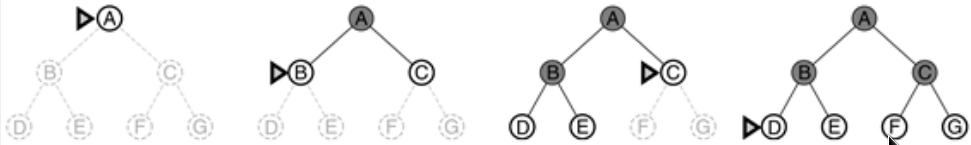
\includegraphics[width=0.8\textwidth]{bfs}
    \caption{Szélességi keresés egy egyszerű bináris fában}
    \label{fig:bfs}
\end{figure}

\subsubsection{Jellemzés}

\begin{itemize}
    \item {\bf Időbonyolultság}: $1 + b + b^2 + \ldots + b^{d+1} - b \in O(b^{d+1})$
    \item {\bf Tárbonyolultság}: $1 + b + b^2 + \ldots + b^{d+1} - b \in O(b^{d+1})$
    \item {\bf Teljesség}: teljes, ha $b$ véges,
    \item {\bf Optimalitás}: optimális, ha minden költség egységnyi.
\end{itemize}

\subsection{Mélységi kereső}

A {\bf mélységi keresés (depth-first search)} mindig a keresési fa aktuális
peremében a legmélyebben fekvő csomópontot fejti ki. A keresés azonnal a fa
legmélyebb szintjére jut el, ahol a csomópontoknak már nincsenek követőik.
Kifejtésüket követően kikerülnek a peremből és a keresés "visszalép" ahhoz a
következő legmélyebben fekvő csomóponthoz, amelynek vannak még ki nem fejtett
követői.

Ez a stratégia egy olyan FA-KERESÉS függvénnyel implementálható, amelynek a
sorbaállító függvénye az {\it utolsónak-be-elsőnek-ki (last-in-first-out,
LIFO)}, más néven verem. A mélységi keresést szokás a FA-KERESÉS függvény
alternatívájaként egy rekurzív függvénnyel is implementálni, amely a
gyermekcsomópontokkal meghívja önmagát.

A mélységi keresés nagyon szerény tárigényű. Csak egyetlen, a
gyökércsomóponttól egy levélcsomópontig vezető utat kell tárolnia, kiegészítve
az út minden egyes csomópontja melletti kifejtetlen csomópontokkal. Egy
kifejtett csomópont el is hagyható a memóriából, feltéve, hogy az összes
leszármazottja meg lett vizsgálva. Egy $b$ elágazási tényezőjű és m maximális
mélységű állapottér esetén a mélységi keresés tárigénye $b\cdot m + 1$.

\subsubsection{Jellemzés (fakeresőként)}

\begin{itemize}
    \item {\bf Időbonyolultság}: $1 + b + b^2 + \ldots + b^m \in O(b^m)$
    \item {\bf Tárbonyolultság}: $1 + b\cdot m \in O(b \cdot m)$, feltéve, hogy
        minden olyan csomópontot elhagyunk, amely összes leszármazottja meg
        lett vizsgálva
    \item {\bf Teljesség}: csak véges körmentes gráfban teljes
    \item {\bf Optimalitás}: nem garantál optimális megoldásokat
\end{itemize}

\subsection{Visszalépéses kereső}

A mélységi keresés {\bf visszalépéses keresésnek (backtracking search)} nevezett
változata még kevesebb memóriát használ. A visszalépéses keresés az összes
követő helyett egyidejűleg csak egy követőt generál.  Minden részben kifejtett
csomópont emlékszik, melyik követője jön a legközelebb. Ily módon csak $O(m)$
memóriára van szükség, $O(b\cdot m)$ helyett. A visszalépéses keresés még egy memória-
(és idő-) spóroló trükkhöz folyamodik. Az ötlet a követő csomópont generálása
az aktuális állapot módosításával, anélkül hogy az állapotot átmásolnánk. Ezzel
a memóriaszükséglet egy állapotra és $O(m)$ cselekvésre redukálódik. Ahhoz, hogy
az ötlet működjön, amikor visszalépünk, hogy a következő követőt generáljuk,
mindegyik módosítást vissza kell tudnunk csinálni. Nagy állapottérrel
rendelkező problémák esetén, mint például robot-összeszerelés esetén, az ilyen
módszerek lényegesek a sikerességhez.

A mélységi keresés hátrányos tulajdonsága, hogy egy rossz választással egy
hosszú (akár végtelen) út mentén lefelé elakadhat, miközben például egy más
döntés elvezetne a gyökérhez közeli megoldáshoz. A legrosszabb esetben a
mélységi keresés a keresési fában az összes $O(b^m)$ csomópontot generálni fogja,
ahol $m$ a csomópontok maximális mélysége. Jegyezzük meg, hogy $m$ sokkal nagyobb
lehet, mint $d$ (a legsekélyebb megoldás mélysége), és korlátlan fák esetén
értéke végtelen.

\begin{megjegyzes}
    A visszalépéses kereső használatával a mélységi keresés tárbonyolultsága
    csökkenthető tovább.
\end{megjegyzes}

\subsubsection{Jellemzés}

\begin{itemize}
    \item {\bf Időbonyolultság}: $1 + b + b^2 + \ldots + b^m \in O(b^m)$
    \item {\bf Tárbonyolultság}: $1 + m \in O(m)$
    \item {\bf Teljesség}: csak véges körmentes gráfban teljes
    \item {\bf Optimalitás}: nem garantál optimális megoldásokat
\end{itemize}

\subsection{Egyenletes költségű (optimális kereső)}

A szélességi keresés optimális, ha minden lépés költsége azonos, mert mindig a
legsekélyebb ki nem fejtett csomópontot fejti ki. Egyszerű általánosítással egy
olyan algoritmust találhatunk ki, amely tetszőleges lépésköltség mellett
optimális. Az {\bf egyenletes költségű keresés (uniform cost search)} mindig a
legkisebb útköltségű $n$ csomópontot fejti ki először, nem pedig a legkisebb
mélységű csomópontot. Egyszerűen belátható, hogy a szélességi keresés is
egyenletes költségű keresés, amennyiben minden lépésköltség azonos.

Az egyenletes költségű keresés nem foglalkozik azzal, hogy {\it hány} lépésből
áll egy bizonyos út, hanem csak az összköltségükkel törődik. Emiatt mindig
végtelen hurokba kerül, ha egy csomópont kifejtése zérus költségű cselekvéshez
és ugyanahhoz az állapothoz való visszatérést eredményez (például a NOOP
cselekvés).

Tegyük fel, hogy előállítjuk az $m$ csomópontot az $n$ csomópont gyermekekeként
és be szeretnénk szúrni az adatbázisba, ahol $m$ már szerepel. Ennek az
útköltségét jelöljük $g(m)$-mel, az újonnan beszúrni kívánt csomópont
útköltségét pedig $g(n)+\text{költség}(\text{operátor})(n)$-nel. Ekkor ha
\begin{itemize}
    \item $g(m) \le g(n)+\text{költség}(\text{operátor})(n)$, akkor az $m$
        csomópontot már sikerült ezelőtt kisebb költséggel előállítani, és nem
        cseréljük le.
    \item $g(m) > g(n)+\text{költség}(\text{operátor})(n)$, akkor az új csúcs
        optimálisabb (tehát nem nagyobb költségű), lecseréljük.
\end{itemize}

A teljességet csak úgy garantálhatjuk, hogy minden lépés költsége
egy kis pozitív e konstansnál nagyobb, vagy azzal egyenlő. Ez a feltétel egyben
az optimalitás elégséges feltétele is.

Ez azt jelenti, hogy egy út költsége az út mentén mindig növekszik. Ebből a
tulajdonságból látszik, hogy az algoritmus a csomópontokat mindig a növekvő
útköltség függvényében fejti ki. Azaz az első kifejtésre kiválasztott
célcsomópont egyben az optimális megoldás is (emlékezzünk arra, hogy a
FA-KERESÉS a célállapottesztet csak a kifejtésre megválasztott csomópontokra
alkalmazza).

Ha $C^*$ az optimális út útköltsége, és minden útköltség legalább $e$,
akkor az időbonyolultság $O(b^{1+(C^*/e)})$.

Mivel az egyenletes költségű kereső mindent csomópontot tárol mindaddig,
amíg megoldást nem talál, a tárigénye a szélességi keresőnél is rosszabb.

Akkor használatos, mikor az útköltségek nem azonosak, amikor azonosak, akkor
BFS-sel is jobban járunk.

\subsubsection{Jellemzés}

\begin{itemize}
    \item {\bf Időbonyolultság}: lehet rosszabb, $O(b^d)$, mert felkutathat
        nagy fákat; $O(b^{1+(C^*/e)})$
    \item {\bf Tárbonyolultság}: $O(b^{1+(C^*/e)})$
    \item {\bf Teljesség}: ha minden lépésköltség egy kis pozitív szám
    \item {\bf Optimalitás}: ha minden lépésköltség egy kis pozitív szám
\end{itemize}

\subsection{Legjobbat először kereső}

Informált keresési módszer.

A {\bf mohó legjobbat-először keresés (greedy best-first search)} azt a
csomópontot fejti ki a következő lépésben, amelyiknek az állapotát a
legközelebbinek ítéli a célállapothoz, abból kiindulva, hogy így gyorsan
megtalálja a megoldást. A csomópontokat az algoritmus tehát az $f(n) = h(n)$
heurisztikus függvénnyel értékeli ki.

A legjobbat-először keresés az általános FA-KERESÉS vagy GRÁF-KERESÉS
algoritmusok olyan speciális esete, ahol egy csomópont kifejtésre való
kiválasztása egy f(n) kiértékelő függvénytől (evaluation function) függ. A
heurisztikáját nézi a csomópontnak, és a kiterjesztett szülőcsomópont, amit lát
az utódokon heurisztika az alapján választja ki a legkisebb heurisztikával
rendelkező gyermeket, és fogja azt kiterjeszteni.

Hagyományosan a legkisebb értékű csomópontot választjuk kifejtésre, mert a
kiértékelő függvény a céltól való távolságot méri.  A legjobbat-először keresés
az eddigi általános keresési eljárások keretein belül egy prioritási sor
segítségével implementálható, ami egy olyan adatstruktúra, mely a peremet a
növekvő $f$-értékek szerint rendezi.

\subsubsection{Jellemzés}

\begin{itemize}
    \item {\bf Időbonyolultság}: $O(b^m)$
    \item {\bf Tárbonyolultság}: $O(b^m)$
    \item {\bf Teljesség}: nem teljes
    \item {\bf Optimalitás}: nem optimális
\end{itemize}

\begin{megjegyzes}
    Az idő- és tárbonyolultság nagyban függ a heurisztikus függvény
    minőségétől.
\end{megjegyzes}

\subsection{Az A* algoritmus}

Informált keresési módszer.

A legjobbat-először keresés leginkább ismert változata az A* keresés. A
csomópontokat úgy értékeli ki, hogy összekombinálja $g(n)$ értékét – az aktuális
csomópontig megtett út költsége – és $h(n)$ értékét – vagyis az adott
csomóponttól a célhoz vezető út költségének becslőjét: \[
    f(n) = g(n) + h(n)
.\]

Mivel $g(n)$ megadja a kiinduló csomóponttól az n csomópontig számított
útköltséget, és h(n) az n csomóponttól a célcsomópontba vezető legolcsóbb
költségű út költségének becslője, így az alábbi összefüggést kapjuk:
\[
    f(n) = \text{a legolcsóbb, az n csomóponton keresztül vezető megoldás
    becsült költsége}
.\]

Így amennyiben a legolcsóbb megoldást keressük, ésszerű először a legkisebb
$g(n) + h(n)$ értékkel rendelkező csomópontot kifejteni. Ezen stratégia
kellemes tulajdonsága, hogy ez a stratégia több mint ésszerű: amennyiben a $h$
függvény eleget tesz bizonyos feltételeknek, az A* keresés teljes és optimális.

\subsubsection{Jellemzés}

\begin{itemize}
    \item {\bf Időbonyolultság}: $O(b^m)$
    \item {\bf Tárbonyolultság}: $O(b^m)$
    \item {\bf Teljesség}: teljes
    \item {\bf Optimalitás}:
        \begin{itemize}
            \item fakeresőként ha $h(n)$ elfogadható heurisztika
            \item gráfkeresőként optimális, ha $h(n)$ konzisztens (vagyis
                monoton), valamint elfogadható heurisztika, azaz soha nem
                becsül felül (ez következik a konzisztenciából)
        \end{itemize}
\end{itemize}

\begin{definicio}
    Heurisztikus függvény.
    Egy $\left<\mathcal{A}, k, \mathcal{C}, \mathcal{O} \right>$
    állapottér-reprezentációhoz megadott heurisztika egy olyan \[
        h : \mathcal{A} \mapsto \mathbb{N} \text{ függvény, melyre }
        \forall c \in \mathcal{C} h(c) = 0
    .\]

    A heurisztika nem más mint egy becslés amely megmondja egy csúcsra nézve,
    hogy melyik gyermeke felé induljon tovább a keresésben. A heurisztikus
    kereső nem teljesen megbízható mivel a részfák még nincsenek legenerálva,
    azaz nem lehetünk biztosak benne.

    Egyes heurisztikákat perfekt heurisztikának nevezünk és egy ilyen
    heurisztika legfeljebb $1+n*d$ csúcsot generál le, azaz ilyen heurisztika
    eseté a csúcsok száma már csak lineáris függvénye a megoldás hosszának.(
    Perfekt heurisztika egyébként nem létezik, mert ha lenne akkor már előre
    ismernénk a megoldást - nem lenne értelme keresni.)
\end{definicio}

\begin{tetel}
    $h(n)$ elfogadható heurisztika, ha soha nem becsli felül az $n$ csomópontot
    keresztül a célállpothoz vezető út útköltségét.
\end{tetel}

\begin{definicio}
    Konzisztencia.
    Azt mondjuk, hogy a $h(n)$ heurisztikus függvény konzisztens, ha minden $n$
    csomópontra és annak egy tetszőleges a cselekvéssel generált minden $n'$
    utódcsomópontjára az $n$ csomóponttól elért cél becsült költsége nem kisebb, mint
    az $n'$ -be kerülés lépésköltsége és az $n'$ csomóponttól elért cél becsült
    költsége: \[
        h(n) \le c (n, a, n') + h(n')
    .\]
    Ez az általános háromszög egyenlőtlenség (triangle inequality) egy formája,
    amely azt fejezi ki, hogy egy háromszög egy oldala sem lehet hosszabb, mint
    a két másik oldal összege.
\end{definicio}
